\documentclass[10pt,a4paper]{article}

\usepackage[a4paper,margin=0.65in]{geometry}
\usepackage{graphicx}
\usepackage{booktabs}
\usepackage{array}
\usepackage{tabularx}
\usepackage{enumitem}
\usepackage{xcolor}
\usepackage{amsmath}
\usepackage{caption}
\usepackage{float}
\usepackage[hidelinks]{hyperref}

\setlength{\parindent}{0pt}
\setlength{\parskip}{3pt}
\setlength{\tabcolsep}{4pt}
\renewcommand{\arraystretch}{1.12}
\captionsetup{font=small,labelfont=bf}
\setlist[itemize]{leftmargin=*,topsep=2pt,itemsep=1pt,parsep=0pt}
\setlist[enumerate]{leftmargin=*,topsep=2pt,itemsep=1pt,parsep=0pt}
\sloppy

\newcommand{\tightsection}[1]{\vspace{6pt}\section*{#1}\vspace{-1pt}}
\newcommand{\tightsubsection}[1]{\vspace{4pt}\subsection*{#1}\vspace{-2pt}}
\newcolumntype{Y}{>{\raggedright\arraybackslash}X}
\newcolumntype{L}[1]{>{\raggedright\arraybackslash}p{#1}}

\begin{document}

\pagenumbering{arabic}
\begin{titlepage}
    \thispagestyle{plain}
    \setcounter{page}{1}
    \centering
    \vspace*{0.8cm}
    
\includegraphics[width=0.70\linewidth]{uofg-logo.png}
    \vspace{1.0cm}

    {\Large \textbf{CSC3106 Cyber Security}\par}
    \vspace{1.2cm}
    {\huge \textbf{Data-Driven Security Analysis and Defensive Response}\par}
    \vspace{0.9cm}
    {\Large \textbf{Team X}\par}

    \vspace{1.5cm}
    \begin{tabular}{llll}
        \toprule
        Name & GUID & SIT ID & Task Distribution \\
        \midrule
        William Oon Zhen Wei & 3070657O & 2401532 & Equal \\
        Kieran Sim & 3070564S & 2403348 & Equal \\
        Tan Bing Kun Terence & 3070672T & 2401883 & Equal \\
        Dui Ru-En Joshua & 3070683D & 2402201 & Equal \\
        \bottomrule
    \end{tabular}

    \vfill
\end{titlepage}

\setcounter{page}{2}
\normalsize

\tightsection{Part 1: Data-Driven Authentication Log Analysis}

\begin{center}
\begin{tabular}{>{\bfseries}rl}
    Assigned Extract: & \texttt{4\_auth.log} \\
    Chosen Asset: & \texttt{backup01} SSH access surface and privileged \texttt{backup} account \\
    Analysis Script: & \texttt{analysis.py} \\
\end{tabular}
\end{center}

\tightsubsection{1. Security Question and Scope}
\textbf{Security question.} What phases of a cyberattack directed at \texttt{backup01} can be reconstructed through SSH authentication and session data within \texttt{4\_auth.log}, and which defensive measures are most critical for securing privileged accounts?

The scope focuses on host \texttt{backup01}, centering on its SSH service and the operational \texttt{backup} user. This account was subjected to intense targeting and demonstrated an accepted login during an attack wave, followed by immediate sudo activity as root. The log period is Jul 06 to Jul 12. Quantitative data and visualisations were derived using \texttt{analysis.py}. The report reconstructs visible attack stages, separates empirical log data from interpretation, and highlights visibility gaps: \texttt{auth.log} cannot prove post-compromise actions such as data exfiltration or system tampering.

\tightsubsection{2. Method Summary}
\texttt{analysis.py} decomposes log entries into syslog components before categorising \texttt{sshd}, PAM, \texttt{sudo}, and CRON messages into security events. It extracts user identities, source IPs, ports, commands, and authentication outcomes, identifies session transitions and privileged command execution, and preserves raw lines for review while maintaining visibility into parsing coverage via separate counts for ambiguous data (refer to Appendix~\ref{app:parsing-coverage}). Because the file lacks strict chronological ordering, timelines are reconstructed from parsed timestamps. Ordering anomalies are retained as investigation limitations, not treated as proof of tampering.

\tightsubsection{3. Evidence Overview}
The extract contains 12,000 lines, all for \texttt{backup01}. Headline counts are shown in Table 1.

\begin{table}[H]
\centering
\caption{Headline counts from \texttt{4\_auth.log}.}
\begin{tabular}{lr@{\hspace{1.0cm}}lr}
\toprule
Event type & Count & Event type & Count \\
\midrule
Failed password & 5,176 & Session opened & 1,047 \\
Accepted password & 1,859 & Session closed & 1,046 \\
Invalid user & 751 & Max auth attempts & 640 \\
Preauth closed & 752 & Sudo command & 255 \\
CRON session & 394 & Possible break-in warning & 80 \\
\bottomrule
\end{tabular}
\end{table}

\begin{figure}[H]
\centering
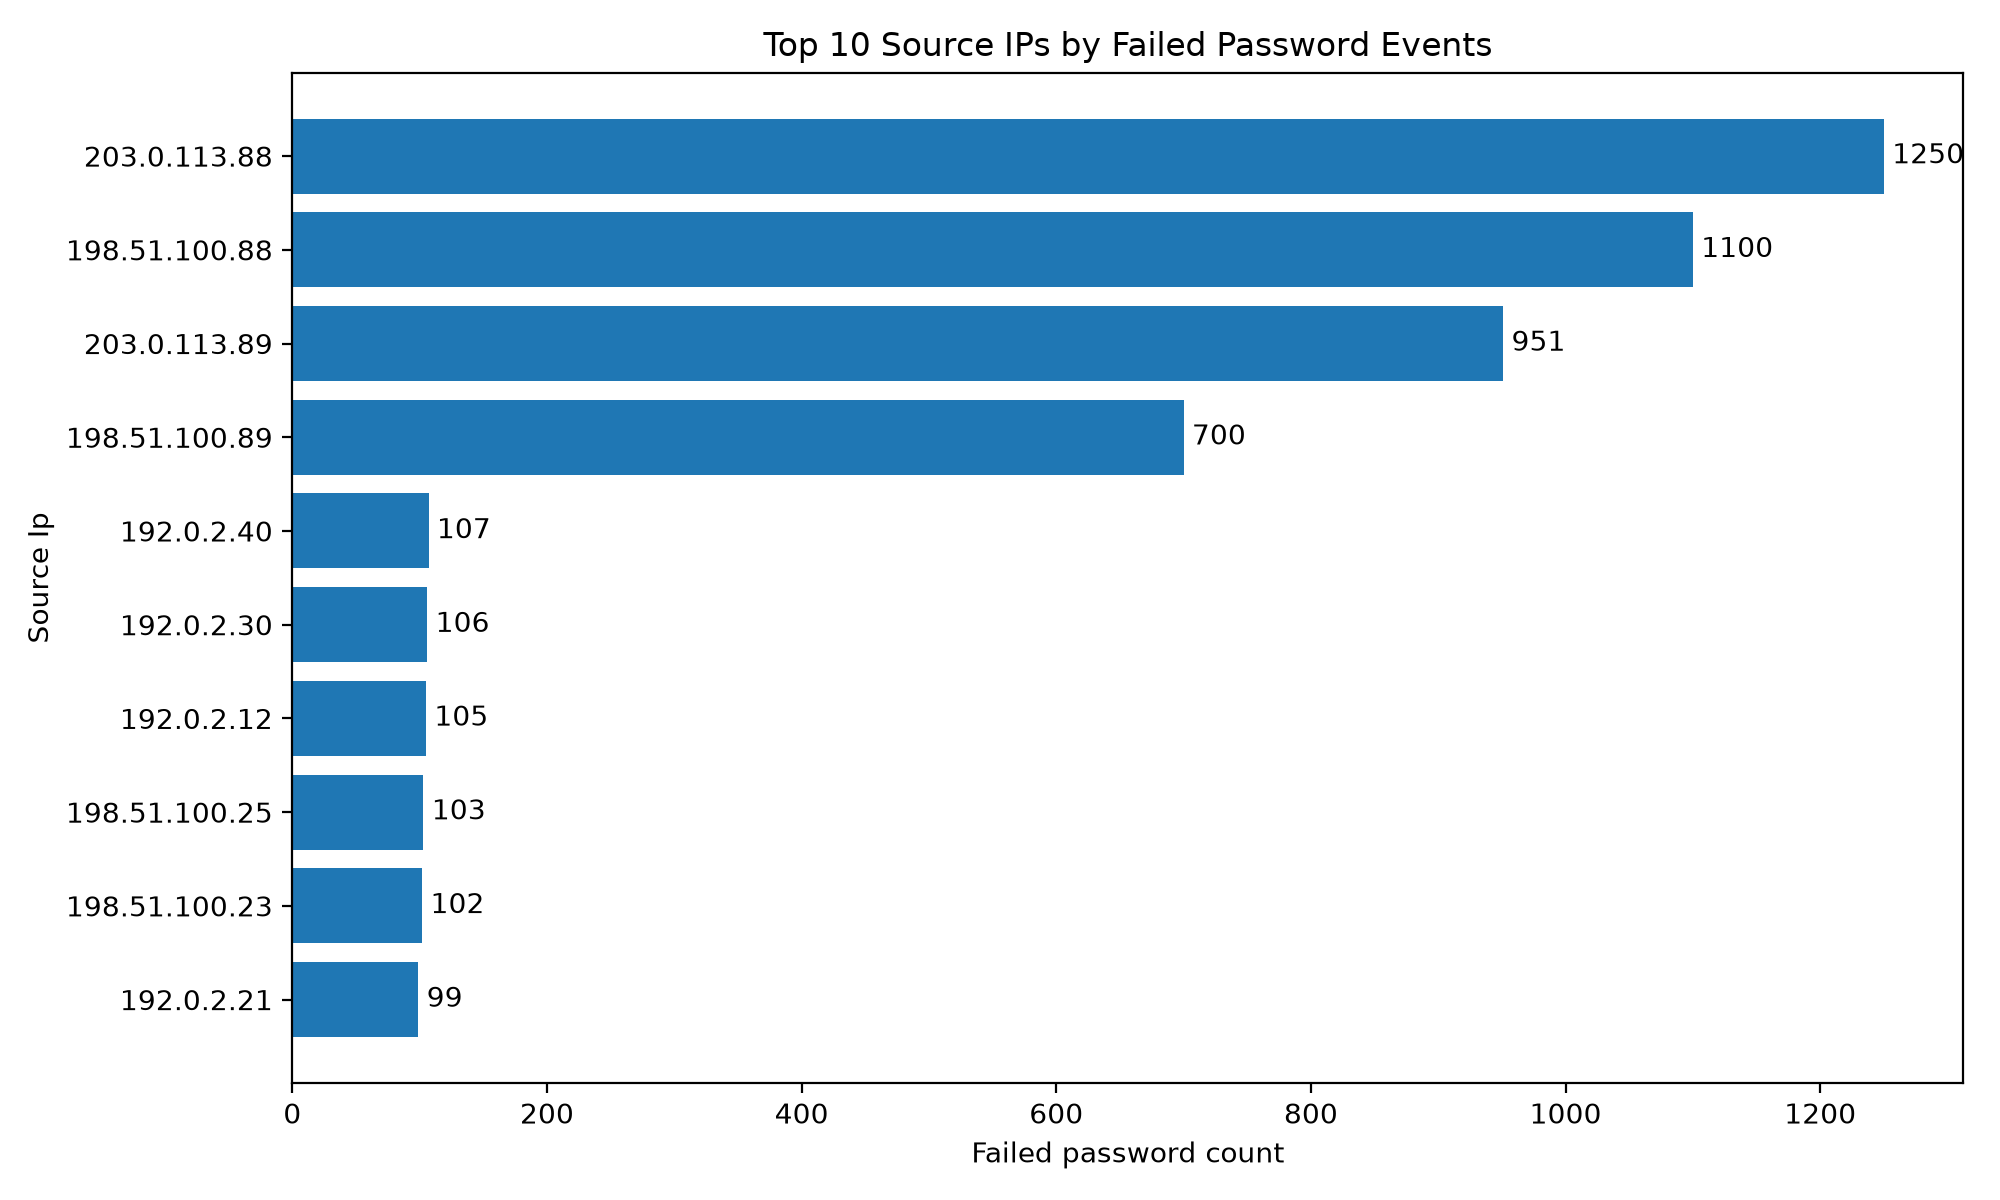
\includegraphics[width=0.76\linewidth]{output/top_source_ips_failed.png}
\caption{Top source IPs by failed password attempts. Four sources dominate SSH failure volume; \texttt{203.0.113.89} is notable because it later records a successful \texttt{backup} login.}
\end{figure}

The high failed-password volume indicates broad SSH credential guessing. Four sources dominate: \texttt{203.0.113.88}, \texttt{198.51.100.88}, \texttt{203.0.113.89}, and \texttt{198.51.100.89}; full counts are in Appendix~\ref{app:evidence-risk}, Table~\ref{tab:app-source-ips}. The username targeting (\texttt{root}, \texttt{admin}, \texttt{deploy}, \texttt{postgres}, \texttt{oracle}) and sustained volume are consistent with automated opportunistic SSH scanning rather than a bespoke campaign. The volume is therefore context, not proof of compromise. What elevates the finding is that \texttt{203.0.113.89} progresses from failures to a successful privileged-account login.

\tightsection{4. Attacker Lifecycle: The \texttt{203.0.113.89} Sequence}

\begin{figure}[H]
\centering
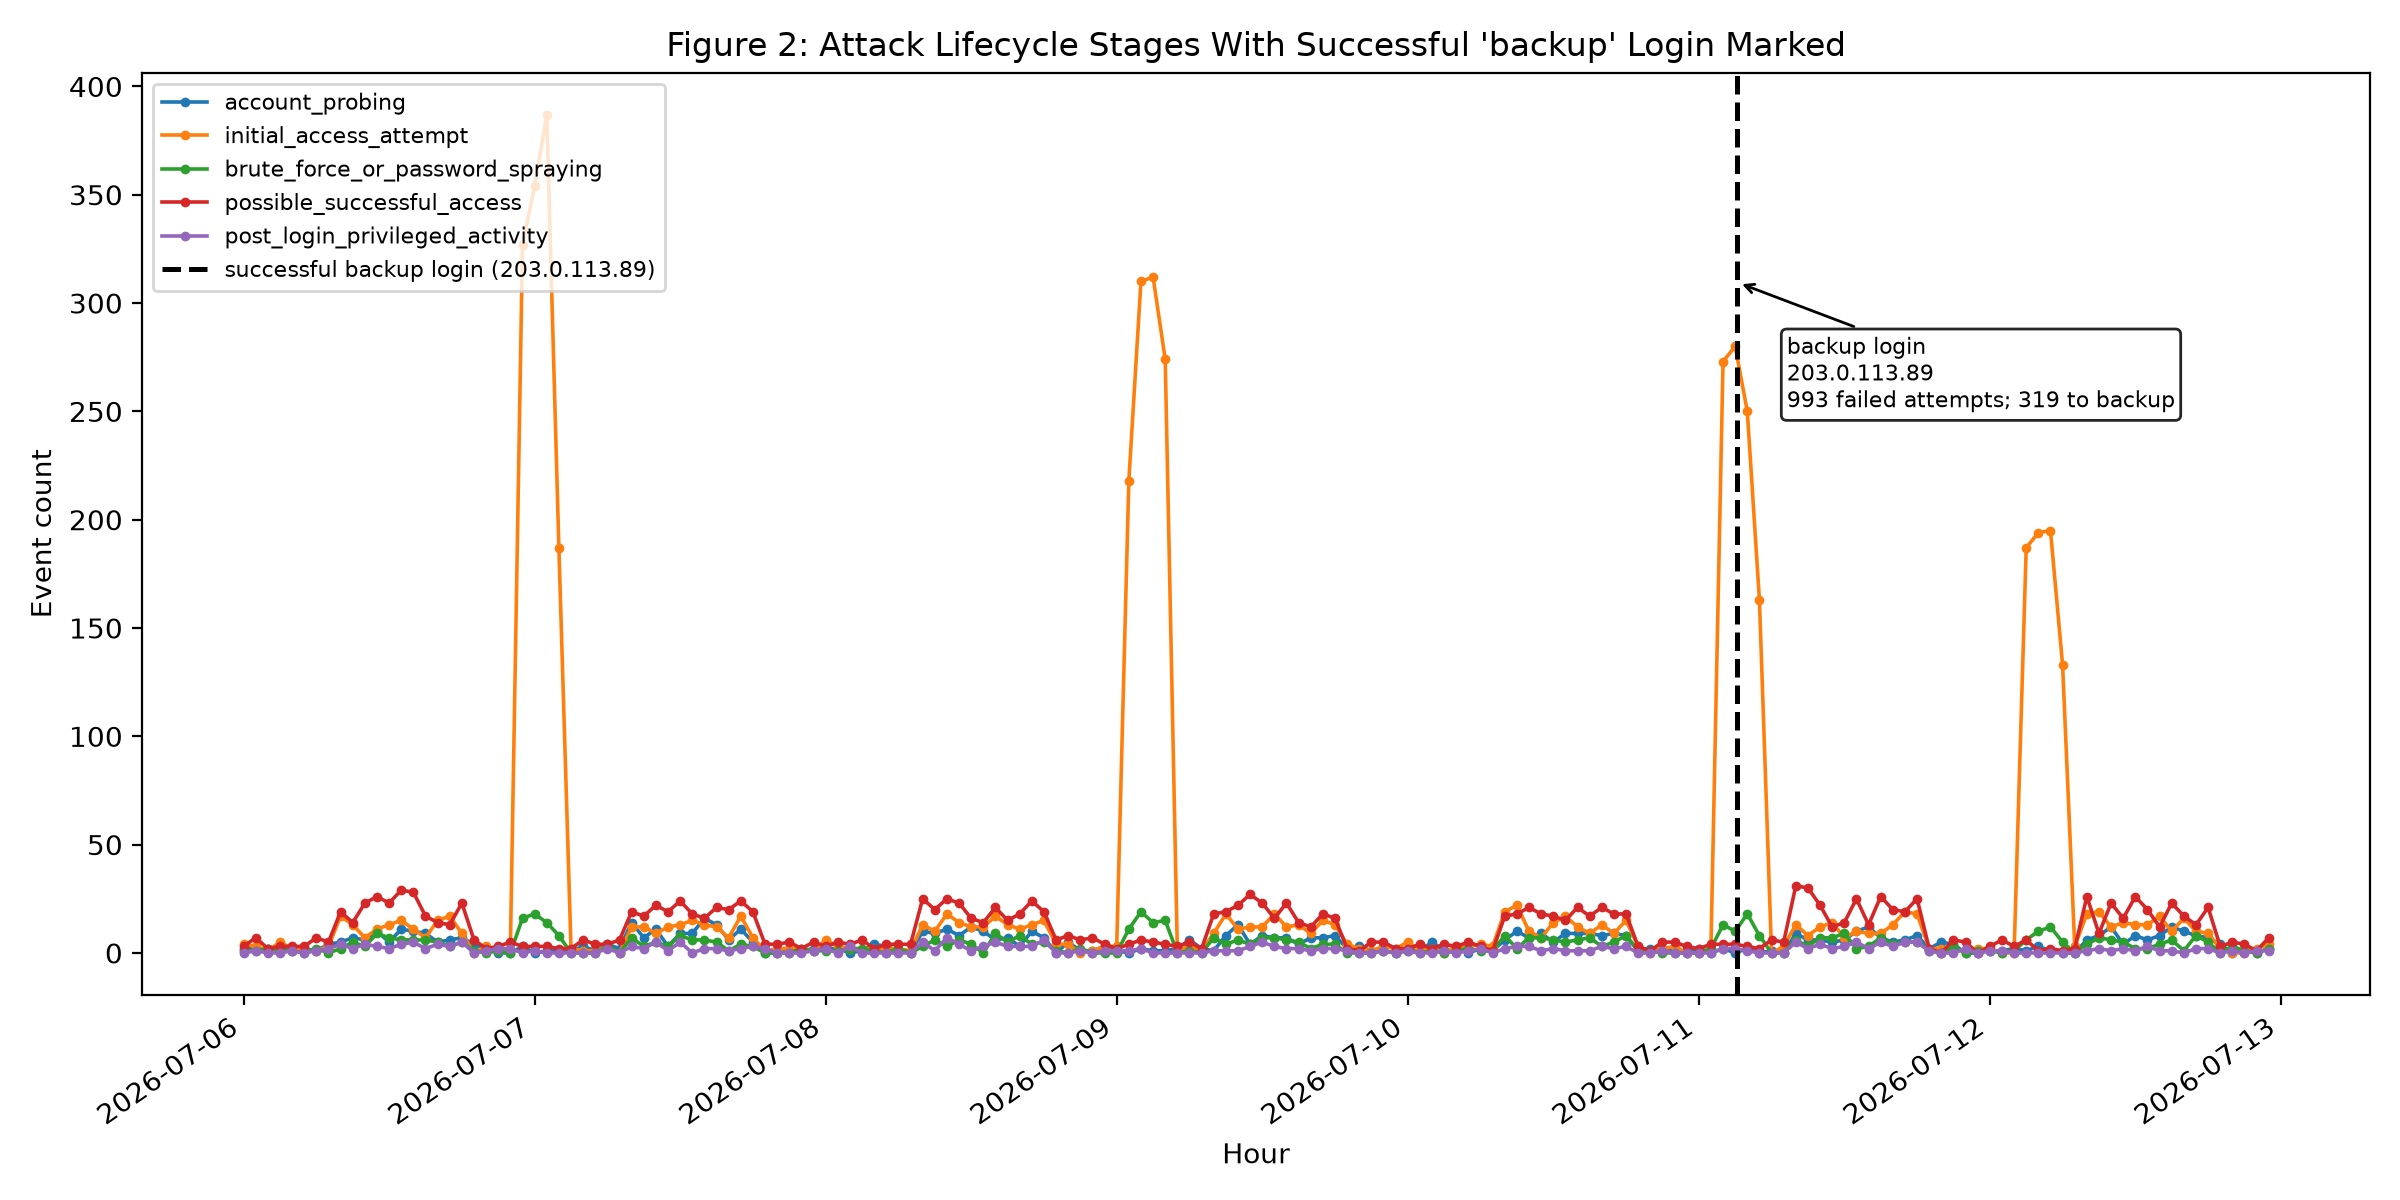
\includegraphics[width=0.86\linewidth]{output/figure2_attack_stages_backup_login.png}
\caption{Attack lifecycle stages over time with the successful \texttt{backup} login marked. The successful login occurs during a major initial-access spike on Jul 11.}
\end{figure}

The strongest finding is a single-source lifecycle on Jul 11. \texttt{203.0.113.89} produced sustained failed attempts and probing, then a successful \texttt{backup} login, an SSH session, and immediate root-level sudo activity.

\begin{table}[H]
\centering
\caption{Critical Jul 11 authentication-to-sudo evidence chain.}
\footnotesize
\begin{tabularx}{\linewidth}{L{1.2cm}Y L{3.0cm}}
\toprule
Time & Evidence and interpretation & ATT\&CK \\
\midrule
03:07:30 & Failed login for invalid user \texttt{oracle} from \texttt{203.0.113.89}; account probing. & T1110.001; consistent with T1087 \\
03:07:32 & Failed password for \texttt{root} from \texttt{203.0.113.89}; privileged-account targeting. & T1110.001 \\
03:08:19 & Accepted password for \texttt{backup} from \texttt{203.0.113.89}; valid-account access over SSH. & T1078; T1021.004 \\
03:08:19 & \texttt{pam\_unix(sshd:session)} opened for user \texttt{backup}; session establishment. & T1021.004 \\
03:08:19 & \texttt{backup} runs \texttt{journalctl -n 200} and \texttt{systemctl status cron} as root; privileged post-login activity. & T1548.003 \\
\bottomrule
\end{tabularx}
\end{table}

The sequence maps most defensibly to T1110.001 $\rightarrow$ T1078 $\rightarrow$ T1021.004 $\rightarrow$ T1548.003: password guessing reaches a valid account over SSH, whose sudo rights expose a path to root. The two sudo commands (\texttt{journalctl}, \texttt{systemctl status cron}) are individually legitimate administrative actions, so they are interpreted as possible privileged reconnaissance immediately after a suspicious login, not confirmed malicious action. Same-second timestamps reflect syslog's one-second precision and do not prove millisecond ordering, but the rapid login-to-sudo transition is more consistent with scripted or prepared activity than routine manual administration. A short raw excerpt is in Appendix~\ref{app:raw-excerpt}.

\textbf{Temporal pattern.} Brute-force activity is concentrated outside working hours: roughly 70\% of failed logins (3,643 of 5,176) fall between 00:00 and 05:59, with a further spike around 23:00. Legitimate accepted logins cluster in business hours (08:00--18:00). In the overnight window there are 3,643 failed against only 149 accepted logins; daytime is close to balanced (1,533 failed vs 1,710 accepted). The successful \texttt{backup} login at 03:08:19 therefore occurs inside the peak attack window and outside the host's normal login baseline, which strengthens the case that it is attacker-driven rather than routine administration (see Appendix~\ref{app:evidence-risk}, Table~\ref{tab:app-time-window}). Host-local time is assumed because no timezone is recorded.

\tightsection{5. Risk Prioritisation}

Asset: \texttt{backup01}, including its SSH access surface, the \texttt{backup} account, and the sudo-to-root path. The three prioritised risks trace the observed attack path: access, escalation, and impact. The full asset-focused risk matrix is included in Appendix~\ref{app:evidence-risk}, Table~\ref{tab:app-risk-matrix}.

R1 is the top priority: it combines attempted access, apparent success, and privileged activity in one source. Secondary risks, including SSH-service degradation from high-volume brute force and exposure of other sudo-capable accounts (\texttt{ops}, \texttt{arun}, \texttt{j.singer}, \texttt{j.maguire}), are noted but not prioritised here. The targeting distribution also supports prioritising the \texttt{backup} account. As shown in Appendix~\ref{app:evidence-risk}, Figure~\ref{fig:app-targeted-users}, \texttt{backup} received the highest number of failed-password and maximum-authentication events among extracted usernames.

\tightsection{6. Initial Response and Investigation Limitations}
Immediate response should verify whether the \texttt{backup} login from \texttt{203.0.113.89} was authorised, rotate or disable the \texttt{backup} credentials until confirmed, preserve relevant logs, and review sudo, cron, journal, shell history, and audit evidence. High-volume SSH sources should also be blocked or rate-limited.

This evidence is limited to \texttt{auth.log}. It shows authentication, session, and sudo activity, but not every shell command. Timestamp-order examples in Appendix~\ref{app:evidence-risk}, Table~\ref{tab:app-timestamp-anomalies} are evidence limitations, not proof of tampering. Therefore, the extract supports likely brute-force activity, possible successful credential compromise, and privileged reconnaissance, but it does not prove botnet activity, malware execution, persistence, exfiltration, log deletion, or destructive tampering. The IP ranges are documentation-style ranges, so no real-world attribution or geolocation should be inferred.

\clearpage
\tightsection{Part 2: Technical Defensive Response}
\textbf{Selected risk.} R1, unauthorised privileged access to \texttt{backup01} via suspected compromise of the \texttt{backup} account, reached through opportunistic SSH brute force from \texttt{203.0.113.89} and extended to root through the account's sudo rights.

\textbf{Defensive goal.} The defence targets the full path rather than brute force alone:
\[
\text{SSH brute-force attempts} \rightarrow \text{successful backup login} \rightarrow \text{active session} \rightarrow \text{sudo as root}.
\]
The response is layered: prevention to stop guessing succeeding, containment to limit damage if a credential is still compromised, and detection to catch a success the preventive layer misses.

\textbf{Cyber Kill Chain framing.} The model is represented as a defensive interruption table for the observed SSH path, not as proof that every Cyber Kill Chain stage occurred.

\begin{center}
\scriptsize
\begin{tabularx}{\linewidth}{L{2.4cm}Y L{2.35cm}L{3.0cm}}
\toprule
Kill-chain stage & Representation in this extract & Evidence status & Defensive interruption \\
\midrule
Reconnaissance & Username and service probing through invalid-user and failed-login attempts. & Visible in \texttt{auth.log}. & Detect abnormal probing and rate-limit repeated failures. \\
Delivery / SSH exploitation & Password guessing against exposed SSH reaches a valid \texttt{backup} login. & Visible as failed passwords followed by accepted login. & Key-only SSH, \texttt{PasswordAuthentication no}, fail2ban/rate limiting, and \texttt{PermitRootLogin no}. \\
Installation/C2 & Malware delivery, persistence, and command-and-control are not visible from this extract. & Not proven by \texttt{auth.log}. & Validate with shell history, full journal, audit logs, cron, and file-integrity review. \\
Actions on objectives / privilege action & Accepted \texttt{backup} login is followed by immediate sudo activity as root. & Suspicious privileged activity, not confirmed damage. & Least-privilege sudoers, SELinux confinement, central logging, and sudo/audit logging. \\
\bottomrule
\end{tabularx}
\end{center}

\begin{table}[H]
\centering
\caption{Recommended controls mapped to observed stages.}
\scriptsize
\begin{tabularx}{\linewidth}{L{2.35cm}L{4.65cm}Y}
\toprule
Attack stage & Control & Security effect \\
\midrule
Password guessing & Key-only SSH; \texttt{PasswordAuthentication no}; rate limiting/fail2ban; \texttt{PermitRootLogin no}. & Password guessing no longer grants access by default; automated brute-force noise is reduced and direct root SSH login is closed. \\
Valid-account SSH access & Restrict the \texttt{backup} key by source and forced command; disable interactive shell if not required. & A stolen password is useless; even a stolen key only runs approved backup operations from approved sources. \\
Privilege escalation via sudo & Least-privilege sudoers for \texttt{backup}; no shell, \texttt{su}, or general sudo. & A compromised \texttt{backup} context cannot obtain a general root shell or run arbitrary privileged commands. \\
Post-compromise tampering & SELinux enforcing, with a confined backup domain. & Limits writes to critical system files, persistence locations, and other paths outside the backup role. \\
Evidence gaps after login & Central log forwarding plus sudo/audit logging. & Preserves evidence beyond local \texttt{auth.log} and gives investigators command-level context after authentication. \\
\bottomrule
\end{tabularx}
\end{table}

\textbf{Evidence-backed Defensive Justification.} The controls are tuned to the observed evidence rather than applied as generic SSH hardening.

\begin{center}
\scriptsize
\begin{tabularx}{\linewidth}{L{4.55cm}Y}
\toprule
Part 1 evidence & Defensive use in Part 2 \\
\midrule
\texttt{backup} is the most targeted account, and \texttt{root} is also heavily targeted (Appendix~\ref{app:evidence-risk}, Figure~\ref{fig:app-targeted-users}). & Justifies key-only SSH for \texttt{backup} and \texttt{PermitRootLogin no}, because both the selected asset account and direct root login are prominent targets. \\
\texttt{203.0.113.89} combines high failure volume, accepted \texttt{backup} login, session establishment, and immediate sudo activity (Appendix~\ref{app:raw-excerpt}). & Justifies prioritising R1 over generic brute-force noise: the concern is the complete access-to-privilege path, not the failure count alone. \\
Night traffic shows 3,643 failed logins against 149 accepted logins (Appendix~\ref{app:evidence-risk}, Table~\ref{tab:app-time-window}). & Justifies off-hours weighting in the alert rule, since the 03:08:19 \texttt{backup} login occurs inside the peak attack window. \\
Other mixed-outcome sources exist, but with much lower failure volume and successful legitimate activity. & Justifies threshold and ratio tuning instead of a naive ``failed then accepted'' rule that would produce false positives. \\
The Jul 11 sequence shows accepted login followed by sudo commands, but \texttt{auth.log} cannot show all shell actions. & Justifies least-privilege sudoers, sudo/audit logging, and central log forwarding to improve containment and investigation beyond local authentication records. \\
\bottomrule
\end{tabularx}
\end{center}

\textbf{Prevention: remove the exposed password surface.} The root cause of R1 is password authentication on a privileged, internet-facing account. Disabling \texttt{PasswordAuthentication} and requiring SSH keys removes the entire brute-force success path; fail2ban-style rate-limiting reduces the noise and load from the ongoing automated scanning identified in Part 1. Denying direct root SSH login closes the most-targeted account (\texttt{root}, 1,048 failed attempts) entirely.

\textbf{Containment: least privilege for the \texttt{backup} account.} Because \texttt{backup} is an operational/service account, broad interactive sudo access is unnecessary risk. Restricting its sudoers entry to the exact commands its backup jobs require, and explicitly denying shell, \texttt{su}, and \texttt{sudo}, prevents a compromised credential from being escalated to a general root shell (the T1548.003 step observed at 03:08:19).

\textbf{Containment: SELinux to protect critical files.} Discretionary permissions and sudo rules can still be bypassed if an attacker reaches root. SELinux in enforcing mode adds mandatory access control: the backup service runs in a confined domain that is permitted to touch only its own data paths. Even a compromised \texttt{backup} context is denied write access to sensitive system files such as \texttt{/etc/passwd}, \texttt{/etc/shadow}, \texttt{/etc/sudoers}, cron directories, and SSH host keys, because those files carry protected types the backup domain has no policy allowance for. This limits both privilege escalation (e.g. editing \texttt{/etc/passwd} or \texttt{sudoers}) and anti-forensic tampering (e.g. altering logs or cron persistence), turning a full host compromise into a contained one.

\textbf{Detection: catching a success the preventive layer misses.} If a credential is still compromised, the failure-then-success transition should raise a high-priority alert. A naive ``failed then accepted from the same IP'' rule is too broad; in this extract 13 source IPs match that pattern, but 12 are legitimate users who occasionally mistype before authenticating (13--28 failures, with successes outnumbering failures). Selectivity therefore comes from tuning to volume and ratio, not the raw pattern. The off-hours concentration from Part 1 also motivates a time-aware detection control: the successful \texttt{backup} login occurred at 03:08:19, inside the 00:00--05:59 peak attack window and outside the host's normal login baseline.

Alert when, from a single source IP within a defined window:
\begin{enumerate}
    \item failed SSH attempts exceed a threshold set above the legitimate baseline; legitimate sources here peaked at $\sim$28 failures, so $\geq$50 cleanly separates them (\texttt{203.0.113.89} produced 311);
    \item and the failure-to-success ratio is heavily skewed (legitimate $\approx$ 1:1; \texttt{203.0.113.89} = 311:1);
    \item and the same IP then obtains an accepted login to the privileged \texttt{backup} account (the only account that successfully authenticates in this log; \texttt{root}, \texttt{admin}, and \texttt{deploy} appear only as failed/invalid targets);
    \item weighted higher when the success and follow-on sudo fall outside business hours (the Part 1 attack window was 00:00--05:59; the compromise was at 03:08).
\end{enumerate}

Applied to this extract, this rule flags \texttt{203.0.113.89} and suppresses the 12 legitimate mixed-outcome sources, giving a high-confidence signal that combines volume, ratio, target sensitivity, and timing.

\textbf{Effectiveness, limitations, and residual risk.} Key-only SSH and root-login denial reduce likelihood by removing the password-guessing success path entirely. Least-privilege sudo and SELinux confinement reduce impact by preventing a compromised \texttt{backup} credential from becoming general root control or tampering with critical files. The tuned correlation rule and central logging improve detection and investigation for any success the preventive layer misses.

\textbf{Limitations and trade-offs.}
\begin{itemize}
    \item Detection selectivity depends on tuning. Thresholds set too low re-introduce the 12 legitimate false positives; too high may miss a low-and-slow attacker. The rule mitigates single-source brute force but not a distributed campaign spread across many IPs.
    \item Rate-limiting/lockout can cause denial of service. Aggressive fail2ban thresholds could block legitimate operations or be abused to lock out accounts; thresholds must be tested so scheduled backup jobs are not interrupted.
    \item Key management overhead. Key-only SSH shifts risk to key storage and rotation; a stolen key still authenticates unless source- and command-restricted.
    \item SELinux is not absolute. Policy authoring and maintenance are non-trivial, mislabelling can break services, and an attacker who reaches an unconfined admin role could still relabel or disable enforcement. It raises the cost of compromise rather than eliminating it.
\end{itemize}

\textbf{Residual risk.} The controls improve prevention, containment, detection, and investigation, but they do not retrospectively prove what happened after the Jul 11 login. Confirming or clearing that event still requires the wider evidence review recommended in Part 1 (shell history, full journal, audit logs, cron and file-integrity checks).

\clearpage
\appendix
\renewcommand{\thetable}{\Alph{section}.\arabic{table}}
\renewcommand{\thefigure}{\Alph{section}.\arabic{figure}}
\setcounter{table}{0}
\setcounter{figure}{0}
\tightsection{Appendices (Supporting Material)}

\section{Supporting Evidence and Risk Matrix}
\label{app:evidence-risk}
\setcounter{table}{0}
\setcounter{figure}{0}

\begin{table}[H]
\centering
\caption{Asset-focused risk matrix for \texttt{backup01}.}
\label{tab:app-risk-matrix}
\scriptsize
\begin{tabularx}{0.9\linewidth}{L{0.55cm}L{2.9cm}L{1.35cm}L{1.1cm}Y}
\toprule
ID & Risk & Likelihood & Impact & Evidence and uncertainty \\
\midrule
R1 & Unauthorised privileged SSH access via suspected \texttt{backup} credential compromise & High & High & 951 failed passwords from \texttt{203.0.113.89}, followed by accepted \texttt{backup} login. Cannot prove whether the login was authorised without external context. \\
R2 & Escalation to root through \texttt{backup} sudo rights & High & Critical & \texttt{backup} runs sudo as root immediately after login. No destructive root command is visible in auth.log. \\
R3 & Loss of backup-data integrity or availability & Medium & Critical & A root path exists on a backup host. Auth.log does not show backup-file access, exfiltration, or tampering. \\
\bottomrule
\end{tabularx}
\end{table}

\begin{table}[H]
\centering
\caption{Top source IPs by failed authentication attempts.}
\label{tab:app-source-ips}
\footnotesize
\begin{tabularx}{0.82\linewidth}{L{3.1cm}rY}
\toprule
Source IP & Failed & Note \\
\midrule
\texttt{203.0.113.88} & 1,250 & High volume; no accepted login \\
\texttt{198.51.100.88} & 1,100 & High volume \\
\texttt{203.0.113.89} & 951 & High volume + one successful \texttt{backup} login \\
\texttt{198.51.100.89} & 700 & High volume \\
\bottomrule
\end{tabularx}
\end{table}

\begin{table}[H]
\centering
\caption{Most-targeted usernames by failed attempts.}
\label{tab:app-targeted-users}
\footnotesize
\begin{tabularx}{0.82\linewidth}{L{3.1cm}rY}
\toprule
Username & Failed & Relevance \\
\midrule
\texttt{backup} & 1,552 & Sensitive; successful login from \texttt{203.0.113.89} \\
\texttt{root} & 1,048 & Direct privileged targeting \\
\texttt{admin} & 589 & Common admin target \\
\texttt{deploy} & 366 & Operational account \\
\texttt{postgres} & 336 & Service/DB account \\
\texttt{oracle} & 331 & Service/DB account \\
\bottomrule
\end{tabularx}
\end{table}

\begin{figure}[H]
\centering
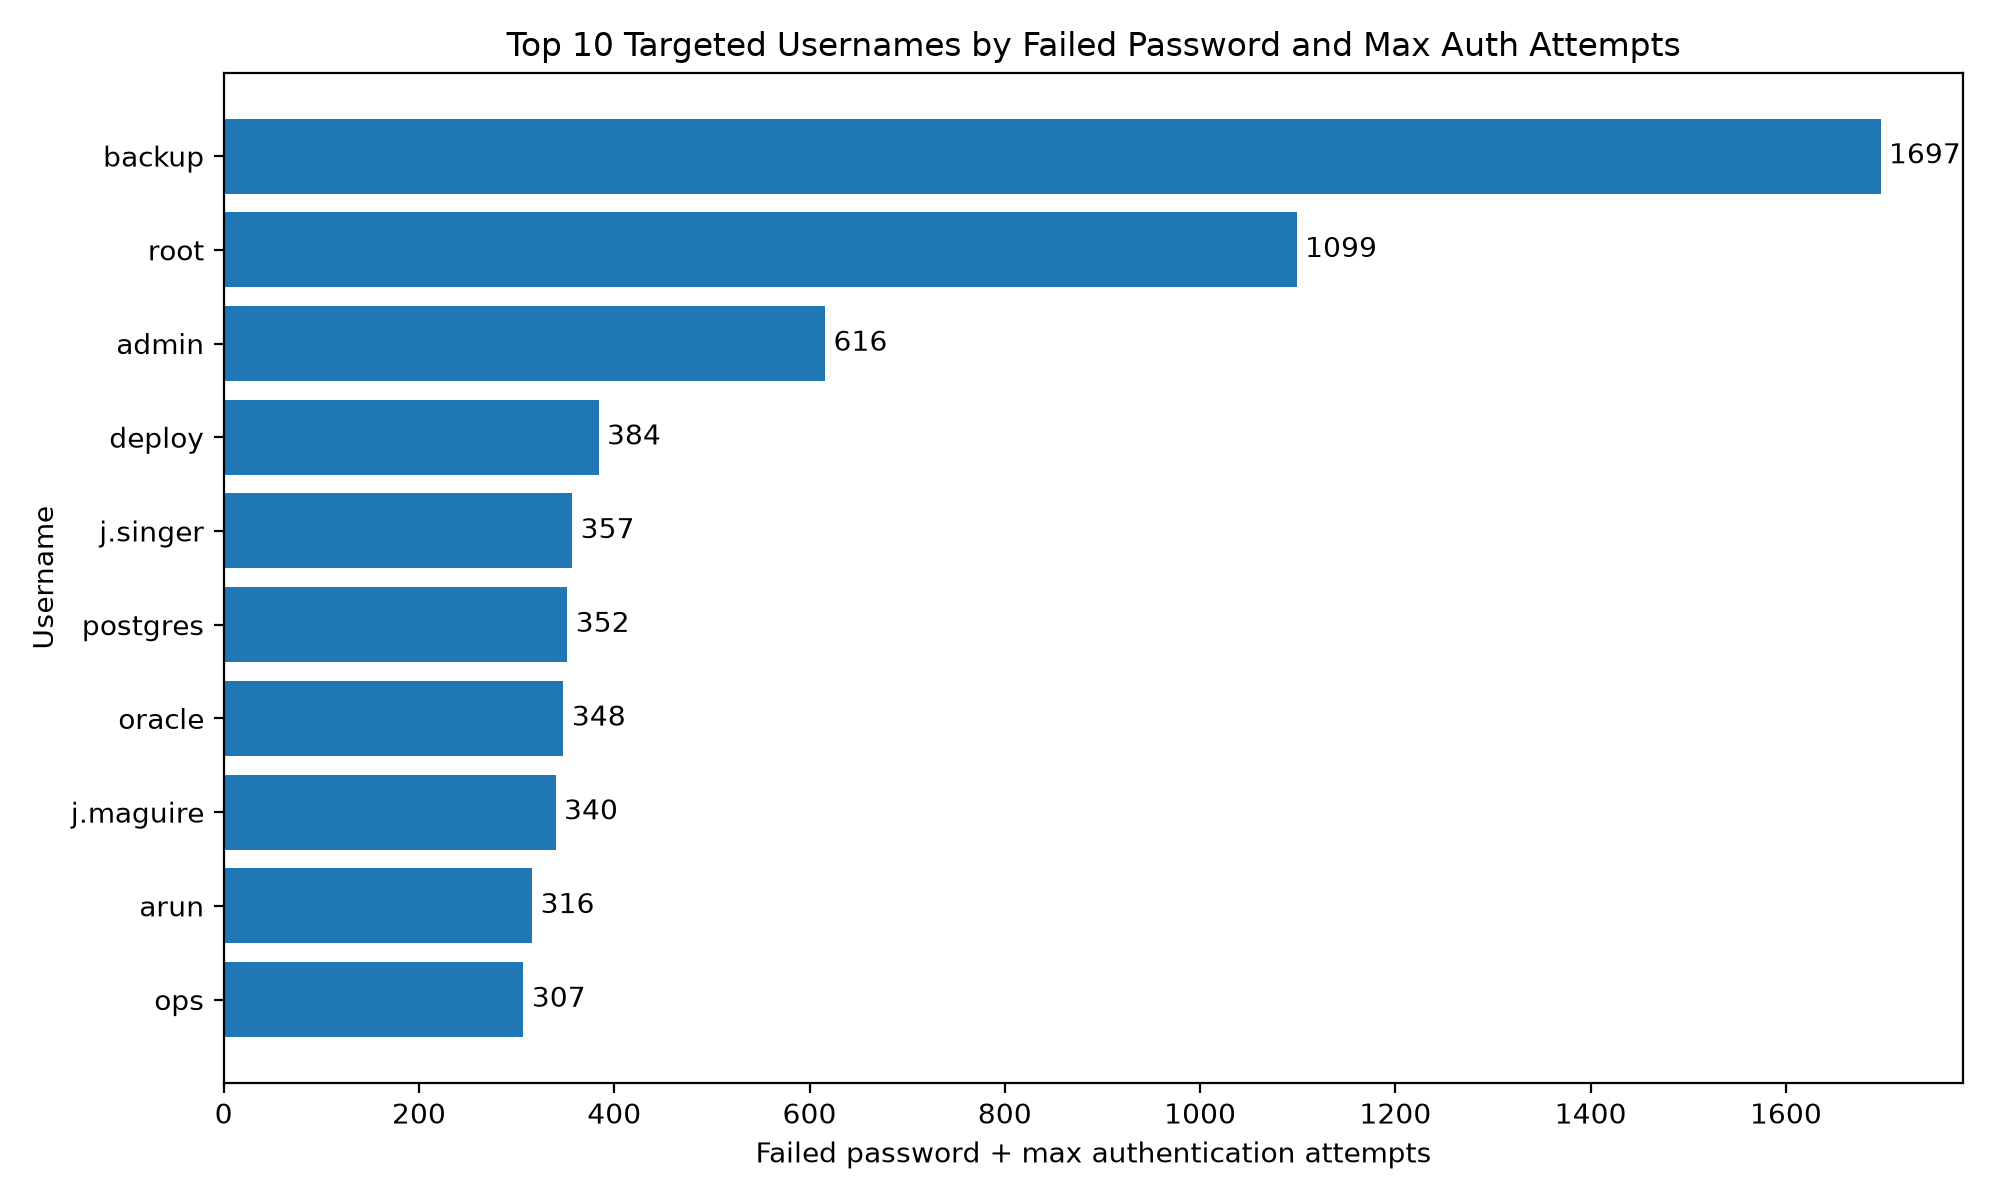
\includegraphics[width=0.62\linewidth]{output/top_targeted_users.png}
\caption{Top targeted usernames by failed-password plus maximum-authentication events. \texttt{backup} is the most targeted account, supporting its selection as the priority privileged asset.}
\label{fig:app-targeted-users}
\end{figure}

\begin{table}[H]
\centering
\caption{Failed vs accepted logins by time window.}
\label{tab:app-time-window}
\footnotesize
\begin{tabularx}{0.82\linewidth}{L{3.0cm}rrY}
\toprule
Window & Failed & Accepted & Note \\
\midrule
Night (00:00--05:59) & 3,643 & 149 & Brute-force concentrated here ($\sim$70\% of all failures) \\
Day (06:00--23:59) & 1,533 & 1,710 & Legitimate activity dominates business hours \\
\bottomrule
\end{tabularx}
\end{table}

Peak failed-login hours are 02:00--04:00; a secondary spike occurs at 23:00. Peak accepted-login hours are 08:00--18:00. The successful \texttt{backup} login (Jul 11 03:08:19) falls inside the peak attack window.

These time-window counts are the Appendix A evidence referenced by the main report for the 03:08:19 off-hours finding.

\begin{table}[H]
\centering
\caption{Timestamp-order anomalies retained as limitations.}
\label{tab:app-timestamp-anomalies}
\footnotesize
\begin{tabularx}{0.9\linewidth}{L{1.0cm}L{2.4cm}L{2.4cm}Y}
\toprule
Line & Previous time & Current time & Interpretation \\
\midrule
13 & 2026-07-06 00:49:51 & 2026-07-06 00:04:24 & Session-close entry appears after later events in file order. \\
41 & 2026-07-06 02:19:09 & 2026-07-06 01:21:46 & Earlier session-close line appears later in the extract. \\
70 & 2026-07-06 03:40:05 & 2026-07-06 02:56:33 & File ordering is not strictly chronological. \\
\bottomrule
\end{tabularx}
\end{table}

\section{Raw Log Excerpt (203.0.113.89, Jul 11)}
\label{app:raw-excerpt}
\setcounter{table}{0}
\setcounter{figure}{0}
\footnotesize
\begin{verbatim}
Jul 11 03:07:30 backup01 sshd[1675]: Failed password for invalid user oracle from 203.0.113.89
port 56854 ssh2

Jul 11 03:07:32 backup01 sshd[1447]: Failed password for root from 203.0.113.89 port 40703
ssh2

Jul 11 03:08:19 backup01 sshd[2164]: Accepted password for backup from 203.0.113.89 port
59595 ssh2

Jul 11 03:08:19 backup01 sshd[7367]: pam_unix(sshd:session): session opened for user backup
by (uid=0)

Jul 11 03:08:19 backup01 sudo: backup : TTY=pts/3 ; PWD=/home/backup ; USER=root ;
COMMAND=/usr/bin/journalctl -n 200

Jul 11 03:08:19 backup01 sudo: backup : TTY=pts/3 ; PWD=/home/backup ; USER=root ;
COMMAND=/usr/bin/systemctl status cron
\end{verbatim}
\normalsize

\section{Parsing Assumptions and Coverage}
\label{app:parsing-coverage}
\setcounter{table}{0}
\setcounter{figure}{0}
\begin{itemize}
    \item Format assumed: Mon DD HH:MM:SS host process[pid]: message; no year in timestamps.
    \item Username handling covers both \texttt{Failed password for USER} and \texttt{Failed password for invalid user USER}.
    \item Non-standard lines (e.g. \texttt{Connection closed by authenticating user ...}, \texttt{reverse mapping ... POSSIBLE BREAK-IN ATTEMPT}) are classified or counted as unmatched, not silently dropped.
    \item Unmatched-line count: 0.
\end{itemize}

\section{AI-Use Declaration and Workload}
\label{app:ai-workload}
\setcounter{table}{0}
\setcounter{figure}{0}
\begin{itemize}
    \item AI-use declaration: Codex GPT-5.5 was used to analyse suspicious points in \texttt{4\_auth.log} so they could be brought to the group's attention for more in-depth analysis. AI was also used to reword and refine the report so that it fits the page limits. Final claims, counts, tables, and figures were checked against \texttt{analysis.py} outputs and the assigned log extract.
    \item Workload record: All members contributed equally.
\end{itemize}

\end{document}
